
\documentclass[11pt]{article}
\usepackage{UF_FRED_paper_style}
\usepackage{listings}
\usepackage{hyperref}
\hypersetup{
	colorlinks=true,
	linkcolor=blue,
	filecolor=blue,      
	urlcolor=blue,
	citecolor=cyan,
}

%% ===============================================
%% Setting the line spacing (3 options: only pick one)
% \doublespacing
% \singlespacing
\onehalfspacing
%% ===============================================

\setlength{\droptitle}{-5em} %% Don't touch

% %%%%%%%%%%%%%%%%%%%%%%%%%%%%%%%%%%%%%%%%%%%%%%%%%%%%%%%%%%
% SET THE TITLE
% %%%%%%%%%%%%%%%%%%%%%%%%%%%%%%%%%%%%%%%%%%%%%%%%%%%%%%%%%%

% TITLE:
\title{COMSM0104: Web Technologies 2019 \\Final Assignment Report}

% AUTHORS:
\author{Tao Xu\\% Name author
	\href{mailto:si19010@bristol.ac.uk}{\texttt{si19010@bristol.ac.uk}} %% Email author 1 
	\and Yinan Yang\\% Name author
	\href{mailto:ff19085@bristol.ac.uk}{\texttt{ff19085@bristol.ac.uk}} %% Email author 2
}

% DATE:
\date{\today}
% %%%%%%%%%%%%%%%%%%%%%%%%%%%%%%%%%%%%%%%%%%%%%%%%%%%%%%%%%%
% %%%%%%%%%%%%%%%%%%%%%%%%%%%%%%%%%%%%%%%%%%%%%%%%%%%%%%%%%%
\begin{document}

	% %%%%%%%%%%%%%%%%%%%%%%%%%%%%%%%%%%%%%%%%%%%%%%%%%%%%%%%%%%
	% %%%%%%%%%%%%%%%%%%%%%%%%%%%%%%%%%%%%%%%%%%%%%%%%%%%%%%%%%%
	% ABSTRACT
	% %%%%%%%%%%%%%%%%%%%%%%%%%%%%%%%%%%%%%%%%%%%%%%%%%%%%%%%%%%
	% %%%%%%%%%%%%%%%%%%%%%%%%%%%%%%%%%%%%%%%%%%%%%%%%%%%%%%%%%%
	{\setstretch{.8}
		\maketitle
		% %%%%%%%%%%%%%%%%%%
		\begin{abstract}
			% CONTENT OF ABS HERE--------------------------------------
			
			Our two-person team consists of Tao Xu (si19010) and Yinan Yang (ff19085). Due to environmental influences, we used a remote collaboration model via GitHub to co-develop this project.
			
			We have created a website that generates resumes. Our website is based on Vue's front-end technical architecture, taking advantage of Vue's MVVM, the Model-View- ViewModel, we have done it to componentize the front-end development.
			
			% END CONTENT ABS------------------------------------------
			\noindent
			\textit{\textbf{Keywords: }%
				Vue; SQLite.} \\ %% <-- Keywords HERE!
			\noindent
			% \textit{\textbf{JEL Classification: }%
			% Q12; C22; D81.} %% <-- JEL code HERE!
			
		\end{abstract}
	}
	
	% %%%%%%%%%%%%%%%%%%%%%%%%%%%%%%%%%%%%%%%%%%%%%%%%%%%%%%%%%%
	% %%%%%%%%%%%%%%%%%%%%%%%%%%%%%%%%%%%%%%%%%%%%%%%%%%%%%%%%%%
	% BODY OF THE DOCUMENT
	% %%%%%%%%%%%%%%%%%%%%%%%%%%%%%%%%%%%%%%%%%%%%%%%%%%%%%%%%%%
	% %%%%%%%%%%%%%%%%%%%%%%%%%%%%%%%%%%%%%%%%%%%%%%%%%%%%%%%%%%
\begin{spacing}{1.0}
	\tableofcontents
	\newpage	
	% --------------------
	\section{Introduction}
	% --------------------
	
	We have created a website that generates resumes called Simple Resume Maker. The website provides basic user registration and login functionality. Once logged in, the user can edit the resume template provided on the website on the web page and download a .pdf version of the resume.
	
	We try to simulate the user experience of editing documents online so that what the user sees is what they get. What would otherwise be a cumbersome formatting process is made easier with different CSS. This addresses the initial point we made in designing the product, which was to make things easier.
	
	In building this site, we used the VUE framework, which is a progressive framework for building user interfaces. 
	
	\begin{center}
		\fbox{\shortstack[l]{
				Unlike other monolithic frameworks, Vue is designed from the ground up to be\\ incrementally adoptable. The core library is focused on the view layer only, and\\ is easy to pick up and integrate with other libraries or existing projects. On the\\ other hand, Vue is also perfectly capable of powering sophisticated Single-Page\\ Applications when used in combination with modern tooling and supporting\\ libraries.\\
				----- Official development documentation from Vue
			}}
		
	\end{center}

	
	\subsection{Project setup}
		npm install
	\subsection{Compiles and hot-reloads for development}
	npm run serve
	\subsection{Compiles and minifies for production}
	npm run build
	\subsection{Lints and fixes files}
	npm run lint
	\subsection{Start the server}
	npm start
	\subsection{Start the server}
	See \href{https://cli.vuejs.org/config/}{Configuration Reference}.
		
	% --------------------
	\section{Self Evalutation}
	\subsection{Estimation of marks}
\begin{itemize}
	\item A for HTML
	\item A for CSS
	\item A for JS
	\item A for PNG	
	\item A for SVG
	\item A for Server
	\item A for Database
	\item A for Dynamic pages
\end{itemize}
	\subsection{Client Side}
	\subsubsection{HTML}
	In terms of front-end architecture, we introduced the Vue architecture, using Vue-CLI as a pre-development generation tool. We chose Vue because we tend to develop a less web-heavy application. If we had used React, it would have been the right choice at some level, but the whole architecture would have been weighty. And that is a departure from the original intent.
	
	For front-end routing, we use vue-route to perform page hops. We compromised on this point because vue is better at performing single-page operations. If you preview our project, you will see that while it looks like we are doing multiple pages, the user is in fact only on one page. We are using routing to control the display of components, which plays to the strengths of vue.
	\begin{figure}[H]
	\centering
	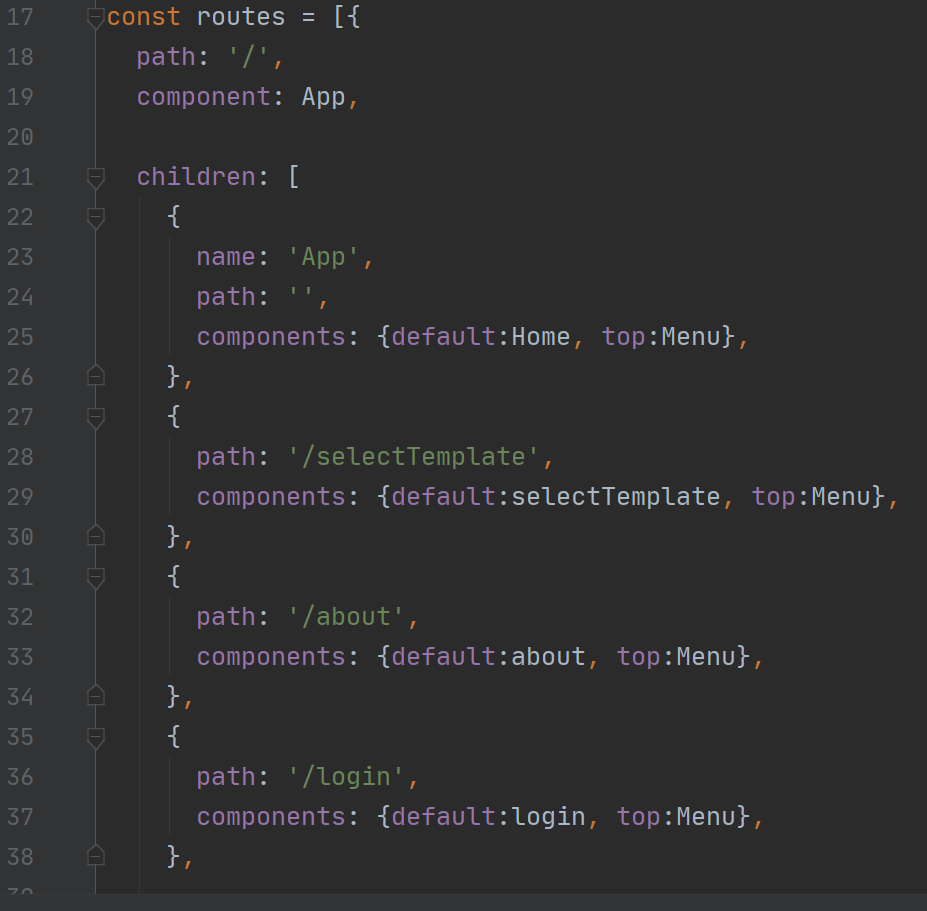
\includegraphics[scale=.3]{figures/routes.png}
	\caption{routes}
	\label{fig:8}
\end{figure}
	
	We completed a total of more than 30 Vue components. Thanks to Vue's component-based development, our front-end applications are not the mess they were a decade ago. Moreover, this design is effortless to maintain later.
	\begin{figure}[H]
		\centering
		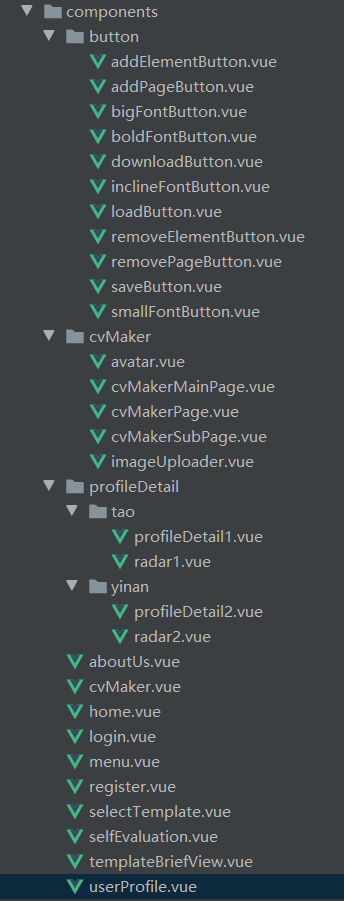
\includegraphics[scale=.5]{figures/components.png}
		\caption{components}
		\label{fig:7}
	\end{figure}

We make full use of the strengths of Vue component communication in the mutual communication of components. Below is an example of a parent component calling a child component method. In the CVMaker page, when we press the bold button in the tools bar and complete the click, the button in an active state.

	\begin{figure}[H]
	\centering
	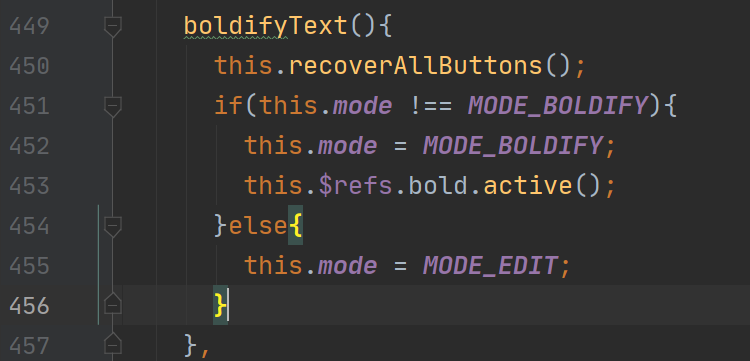
\includegraphics[scale=.3]{figures/componentsRefs.png}
	\caption{component communication}
	\label{fig:9}
\end{figure}
	\subsubsection{CSS}
	We use a separate CSS file that is loaded inside the Vue component. Although the Vue template allows us to define styles internally using the <style> tag, we still load all the CSS placed separately under the folder $src/view/index/assets$ for easy management. For CSS, we have three instructions.
	\begin{itemize}
		\item Use of basic CSS and changing style dynamically by changing style parameters.\\
		Each CSS file contains multiple class ids that are used on specific pages. We also set up a global background CSS, one with a furry glass effect to give the whole screen more colour.
		
		The following is an example of how to adjust the progress bar according to the download progress in the downloadButton. We dynamically adjust the width of the bar to match the expected download. Of course, to avoid single-threaded js blocking, we set a timer to control how often the progress bar refreshes.
\begin{figure}[H]
	\centering
	
\includegraphics[scale=.5]{figures/css.png}
	\caption{change style}
	\label{fig:10}
\end{figure}

\item SVG-based animation\\
 We completed the svg-based animation in CSS, which is also explained in detail in the SVG section.
 \begin{figure}[H]
 	\centering
 	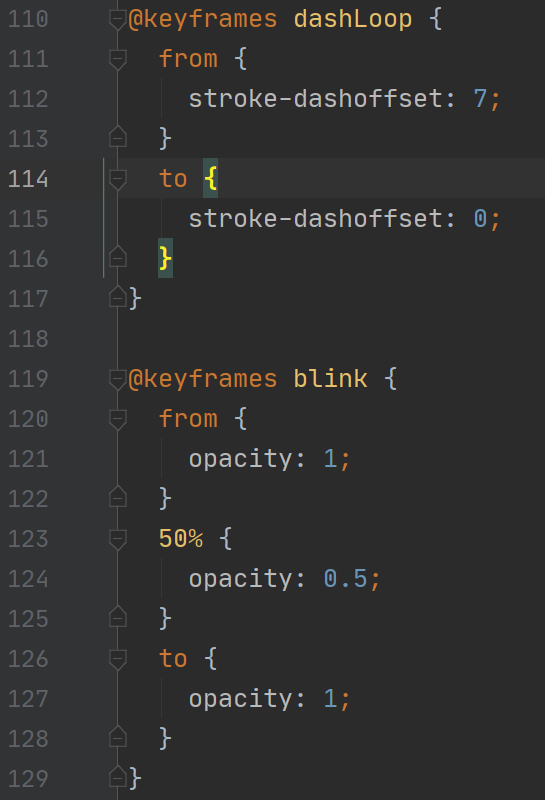
\includegraphics[scale=.5]{figures/cssAnimation2.png}
 	\caption{css animation}
 	\label{fig:11}
 \end{figure}
\item Store CSS in the back-end database for dynamic retrieval\\
The main feature of our website, making different templates for resumes is based on the replacement of different CSS. This is the main logic behind the primary function of our website. In CVMaker, we dynamically retrieve the CSS stored in the database according to the user's choice, to generate the user's Selected resume template. This feature set makes it easier to run this system, maintain it later, and increase the number of resume templates without spending vast resources.
 \begin{figure}[H]
	\centering
	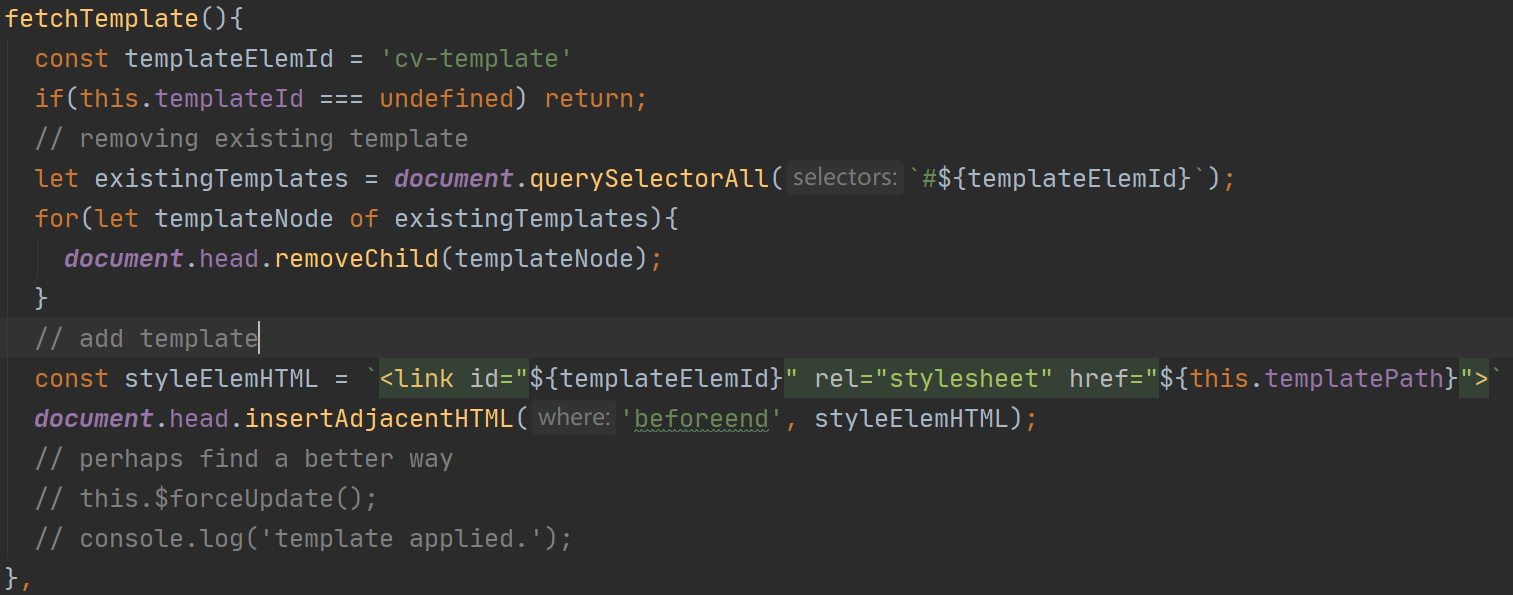
\includegraphics[scale=.4]{figures/cssTemplate.png}
	\caption{resume template}
	\label{fig:12}
\end{figure}
		
	\end{itemize}
	\subsubsection{JS}Because of the vue template, it becomes straightforward to embed js in the page. Each page component exists separately as an element, and we write js methods internally or externally that can change the arithmetic. Of course, this is not technically a javascript file anymore, but primarily at the developmental level, they are a kind of Stuff.
	
	We wrote a lot of front-end and back-end js logic to ensure that the complete project documentation worked adequately. Similar to the button or switch screen functions are used to implement the vue methods. The example below is the js method after the download button is pressed.
	 \begin{figure}[H]
		\centering
		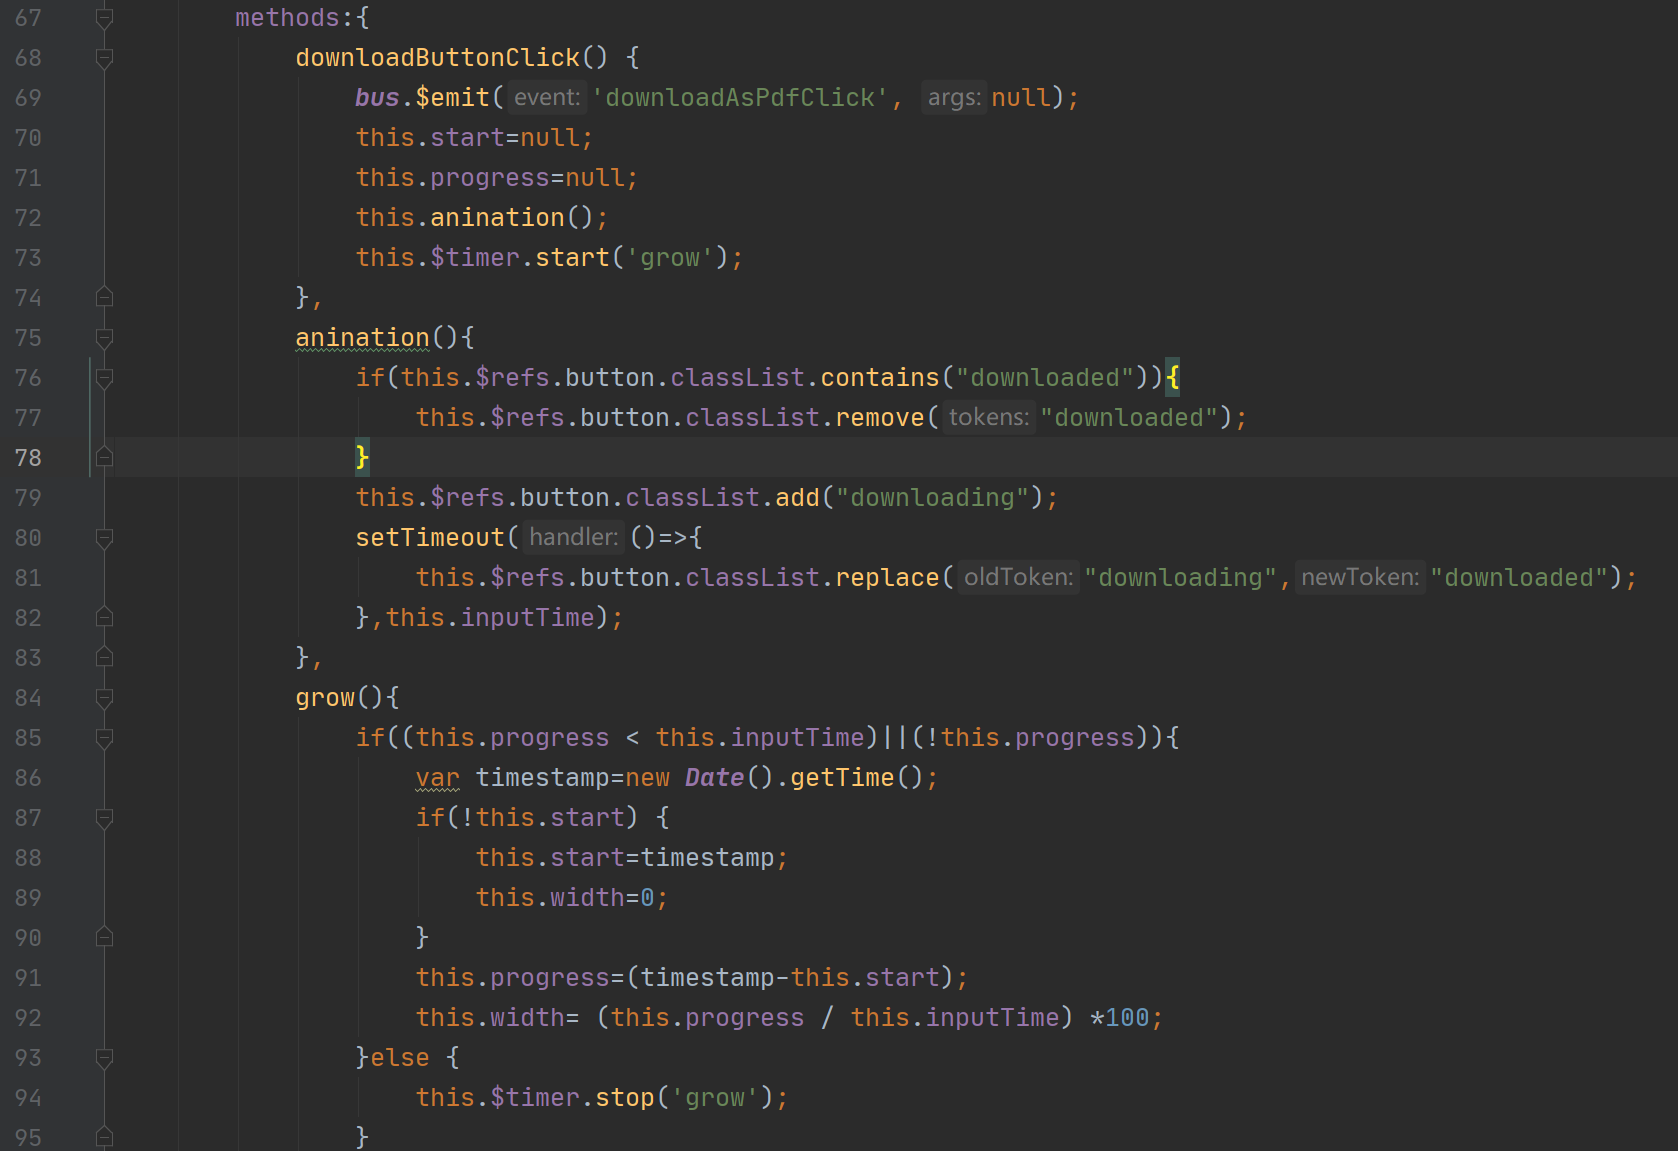
\includegraphics[scale=.4]{figures/downloadButtonJS.png}
		\caption{resume template}
		\label{fig:14}
	\end{figure}
	\subsubsection{PNG}
	We used GMIP for mapping, including the default resume header and png diagrams for 404 pages. The source file of the 404 page is saved in $src/view/index/img$. We used masks, filters and transparent alaph channels, among other techniques.
	\begin{figure}[H]
		\centering
		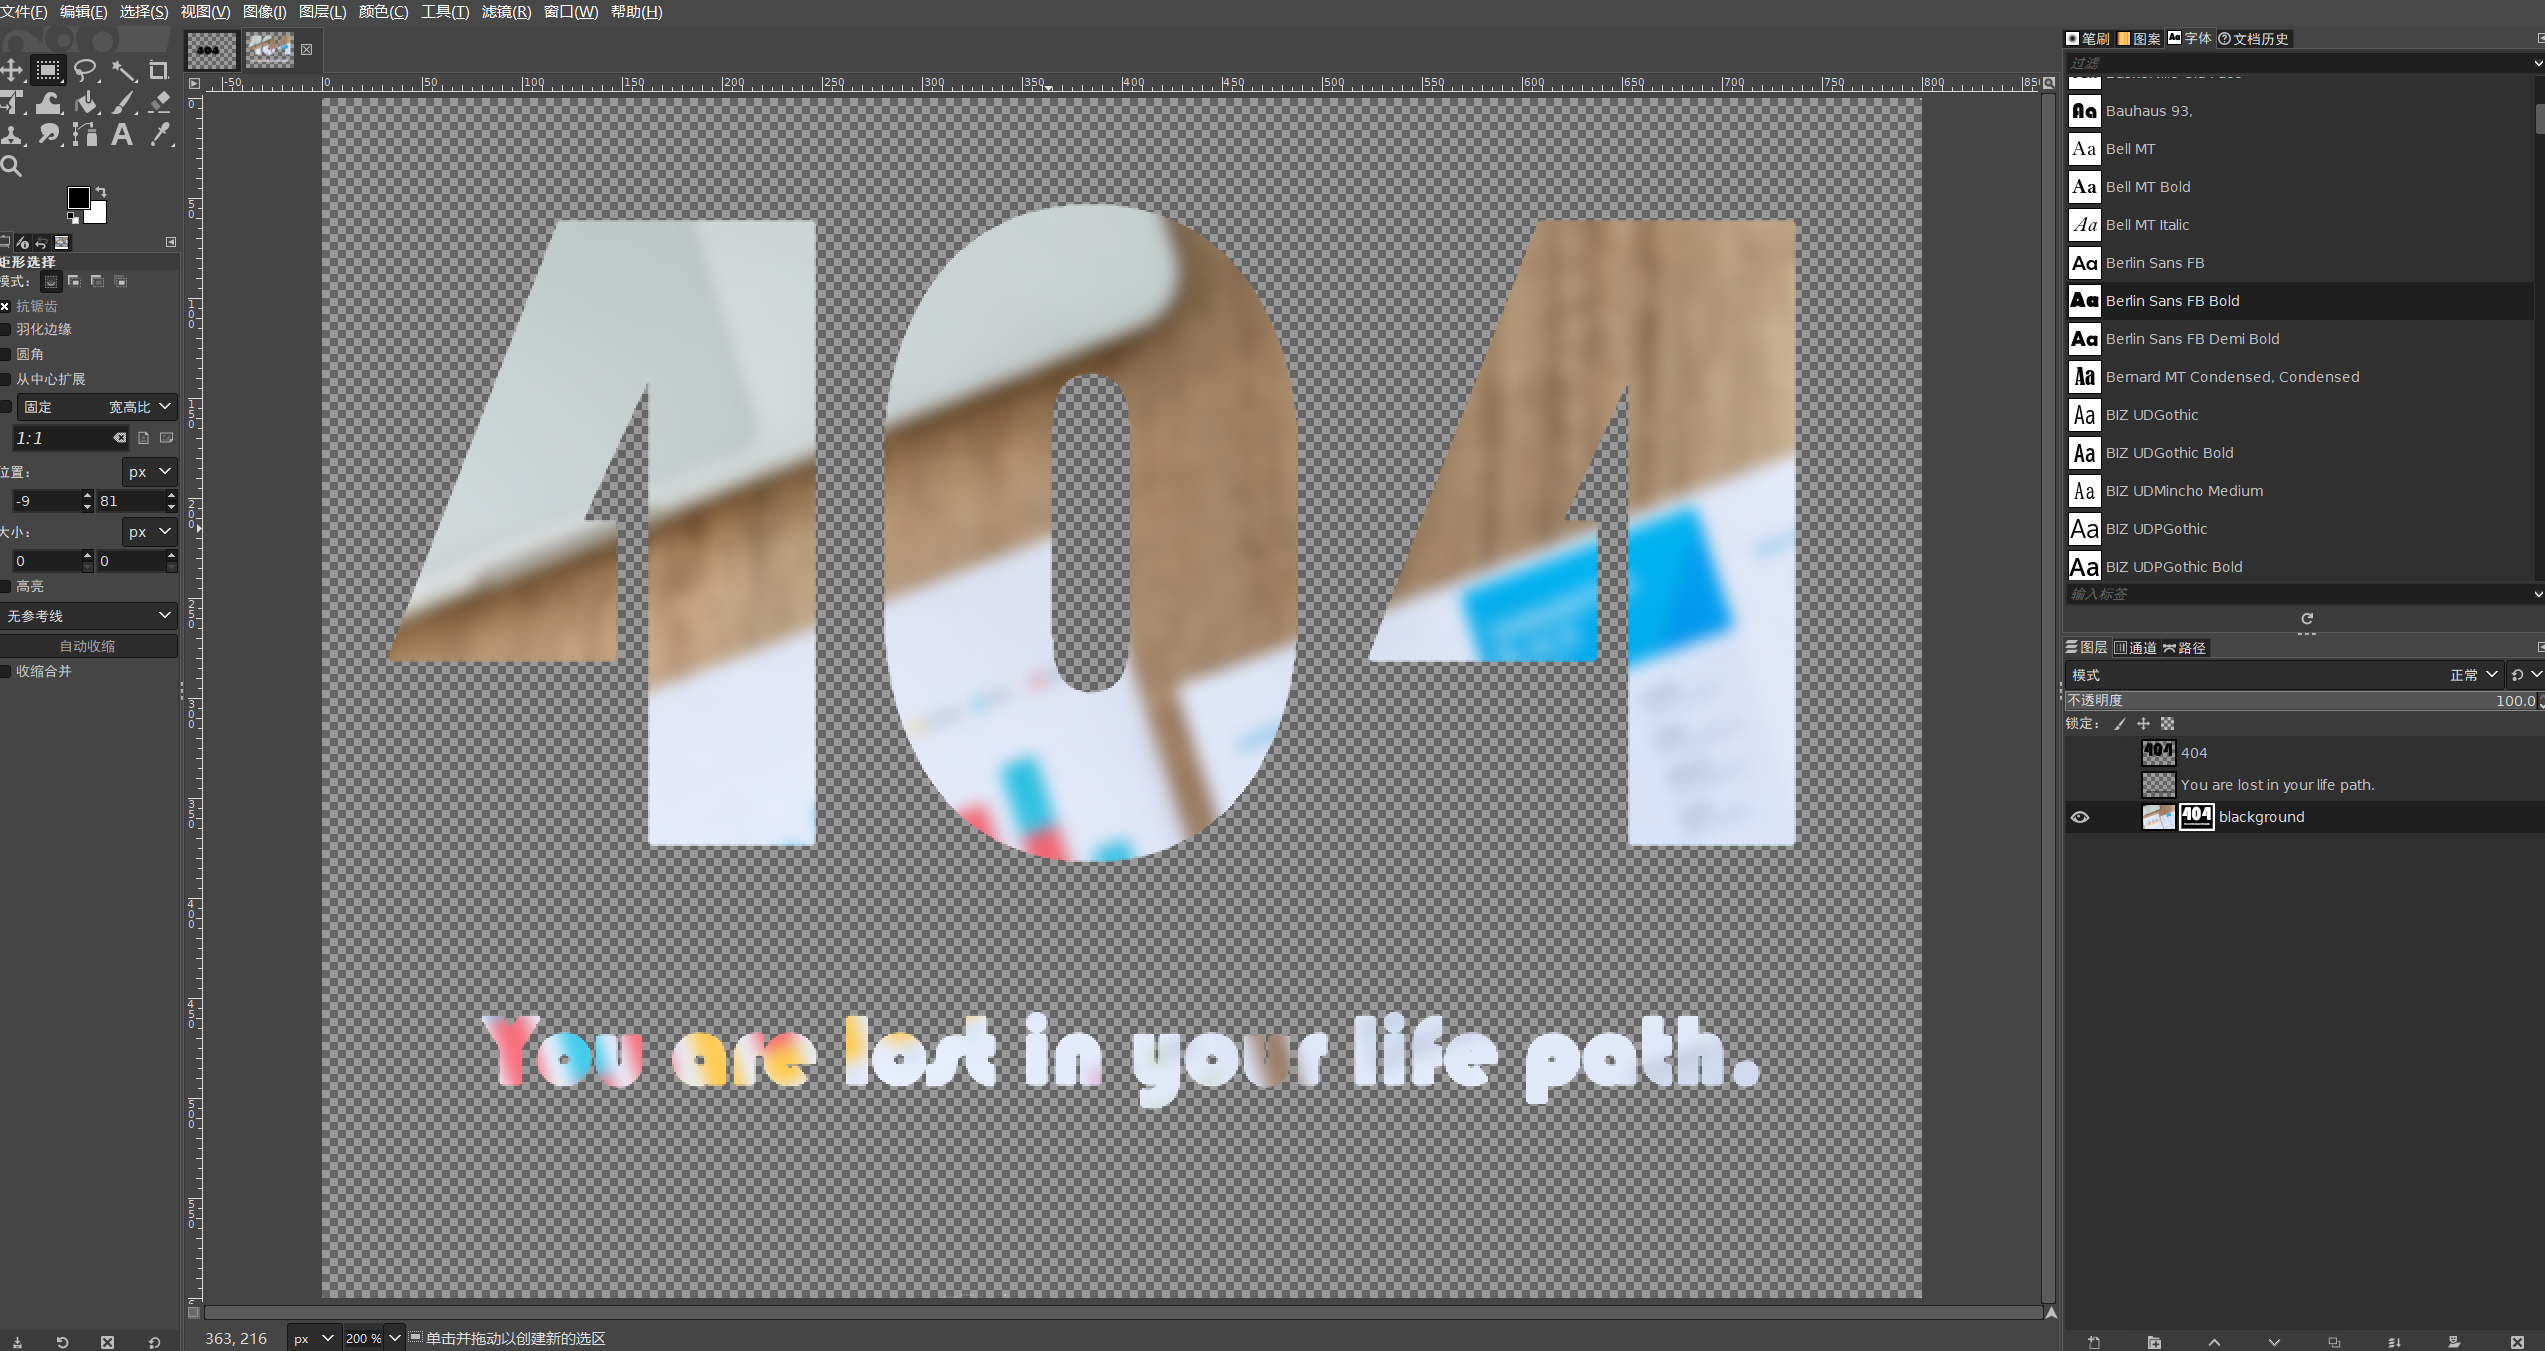
\includegraphics[scale=.3]{figures/404.png}
		\caption{404.png}
		\label{fig:13}
	\end{figure}
	
	\subsubsection{SVG}
	In the use of SVG, we have used a variety of ways to construct SVG images to take full advantage of his benefits. We even created SVG  animation on the home page. We will describe this in detail below.
	\begin{itemize}
		\item Basic SVG images\\
		We used tools like Inkscape to draw simple SVG portraits, and since the team has the skills to operate adobe Kit experience, so we are light on SVG production. 
		\begin{figure}[H]
			\centering
			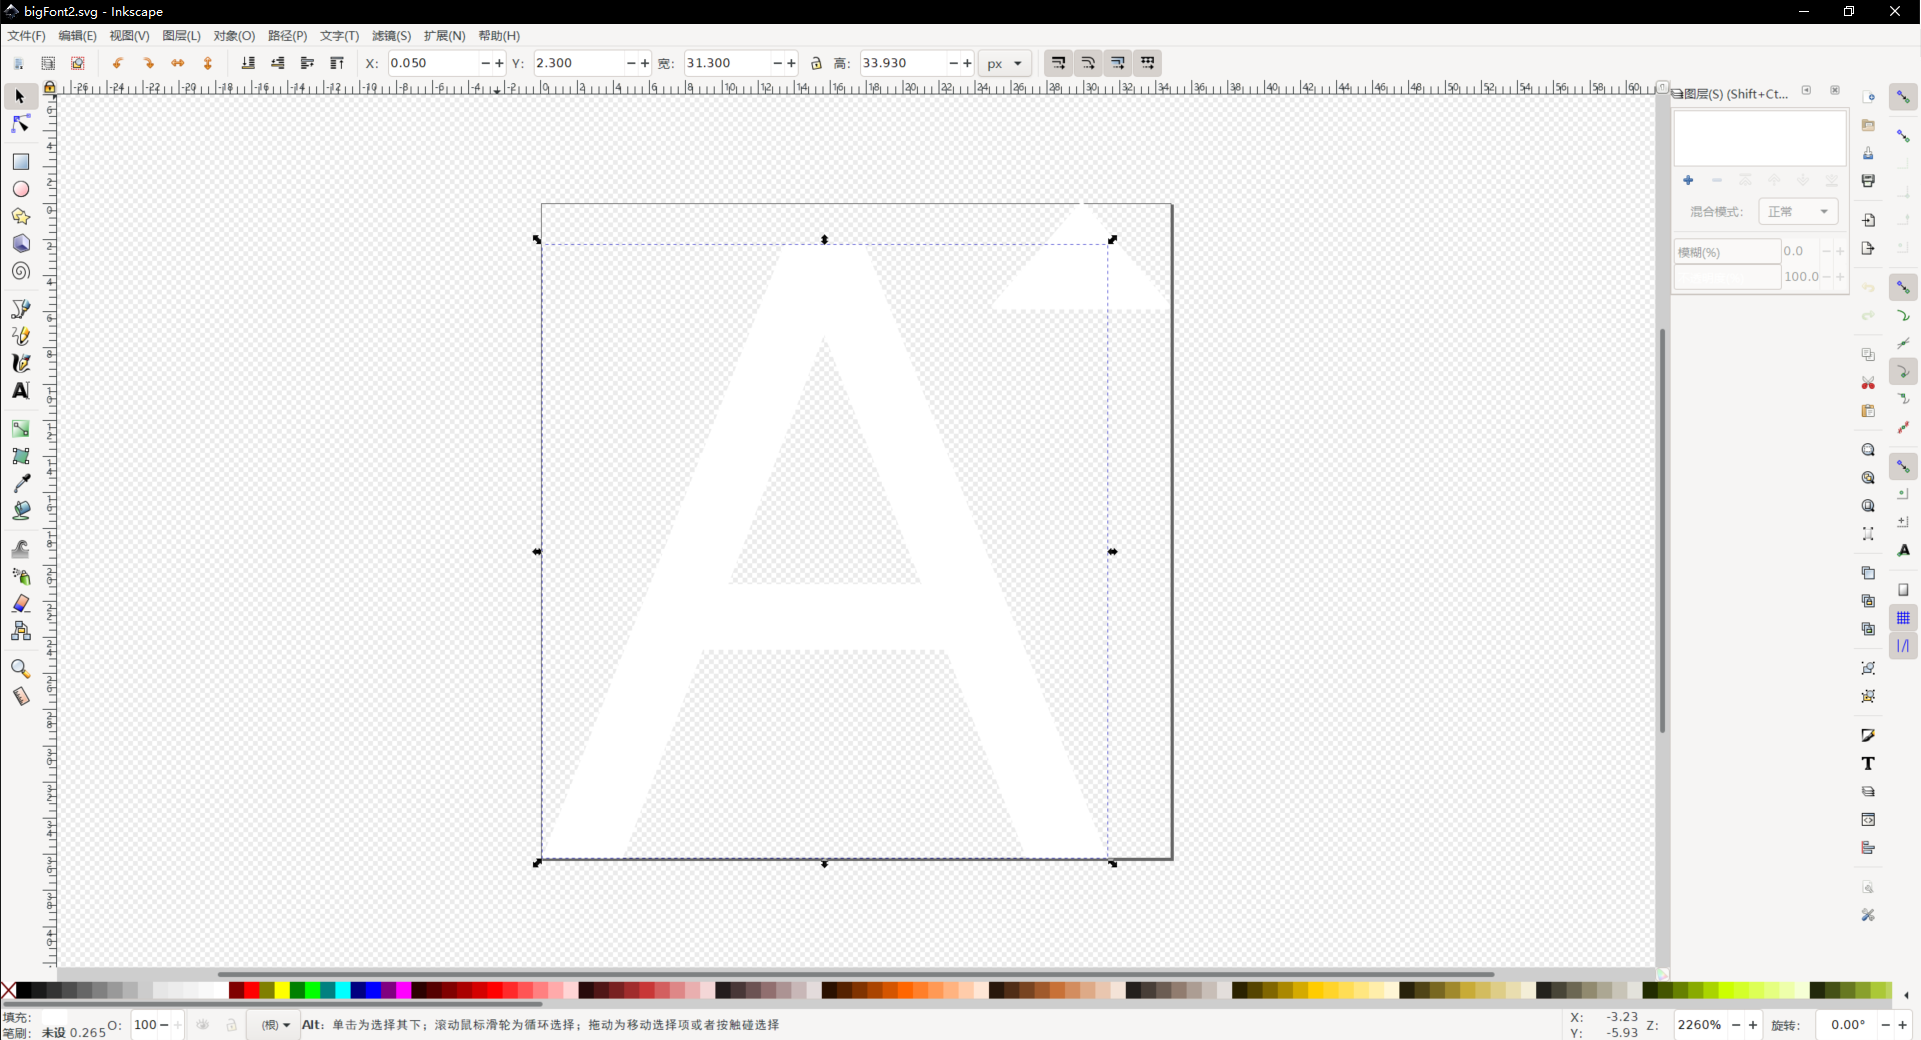
\includegraphics[scale=.3]{figures/svg1.png}
			\caption{Inkscape}
			\label{fig:1}
		\end{figure}
	We used this basic graphical drawing to create 12 buttons, 3 of which are embedded in the page, while the remaining nine are used as Individual components are independent of the elements in the $src/components/button$. We take advantage of the object-oriented component design of the Vue components so that each module is easy to maintain and update later.
	\begin{figure}[H]
		\centering
		
\includegraphics[scale=.3]{figures/buttonBar.png}
		\caption{buttonBar}
		\label{fig:2}
	\end{figure}
	\begin{figure}[H]
	\centering
	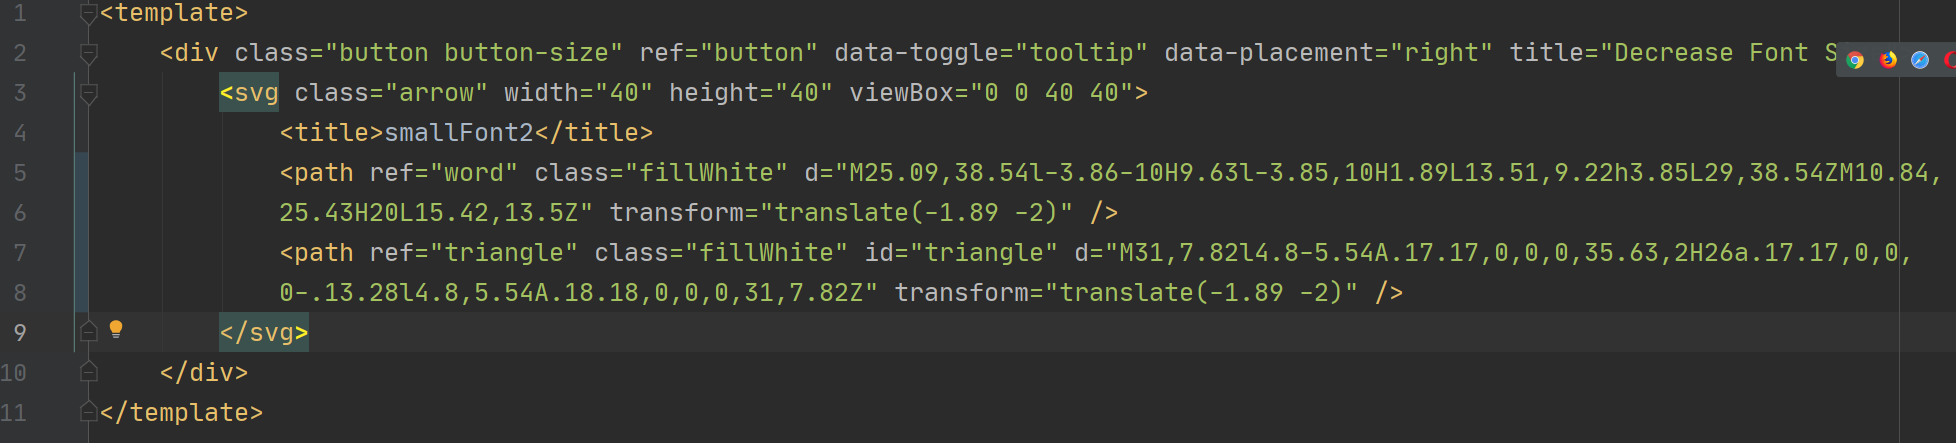
\includegraphics[scale=.3]{figures/smallFontButton.png}
	\caption{smallFontButton}
	\label{fig:3}
\end{figure}
\item SVG-based css animation\\
We were not satisfied with making basic SVG graphics. We created four SVG animations with CSS animation effects. They are the start button on the home page, the continue and new buttons on the user-profile page, and the download button inside CVMaker. The most complex one is the download button, which activates the animation by changing the button's class when clicked. 
\begin{figure}[H]
	\centering
	
\includegraphics[scale=1]{figures/downloadButton.png}
	\caption{downloadButton animation}
	\label{fig:4}
\end{figure}
The download animation is divided into four parts, the first is the flashing of the outer ring, the second is the downward movement of the vertical line in the middle, and the third is the download of The middle arrow pattern becomes a checkmark when finished, and the fourth is the download progress bar at the bottom.
\begin{figure}[H]
	\centering
	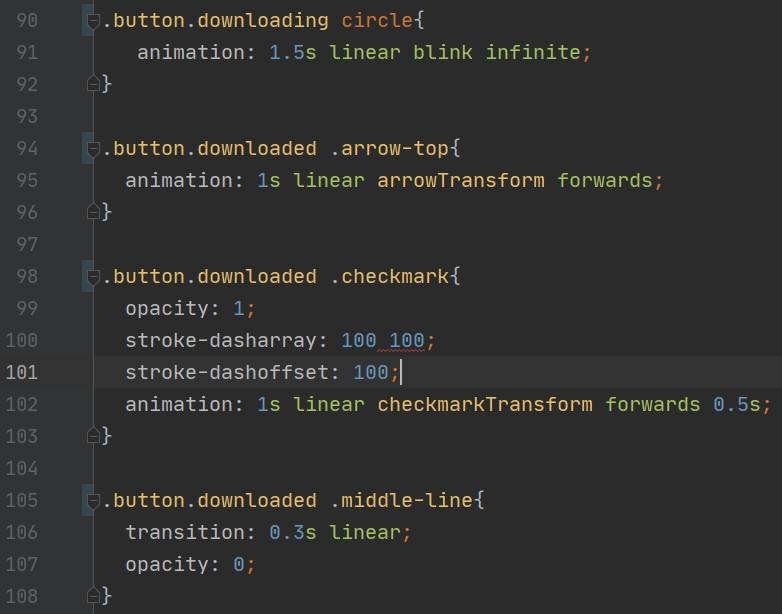
\includegraphics[scale=0.5]{figures/cssAnimation.png}
	\caption{downloadButton animation}
	\label{fig:5}
\end{figure}
\item svg animation based on vue-lottie\\
Of course, doing this will not satisfy our ambition to try the coolest animations. So we introduced the vue-lottie open-source package, which is based on the \href{https://github.com/airbnb/lottie-web}{lottie}. Vue-lottie project vue architecture lottie can be interpreted as an SVG animation interpreter, and he supports the use of SVG in adobe After Effects exports complex animations to a JSON file and then self-rendering through the front-end of the web page to get cool effects.

We've made a dynamic animation on the home page to highlight our theme, which we're sure you've seen.We save the exported animation JSON file that we send to AE in the $src/view/index/assets/animation$ folder.
\begin{figure}[H]
	\centering
	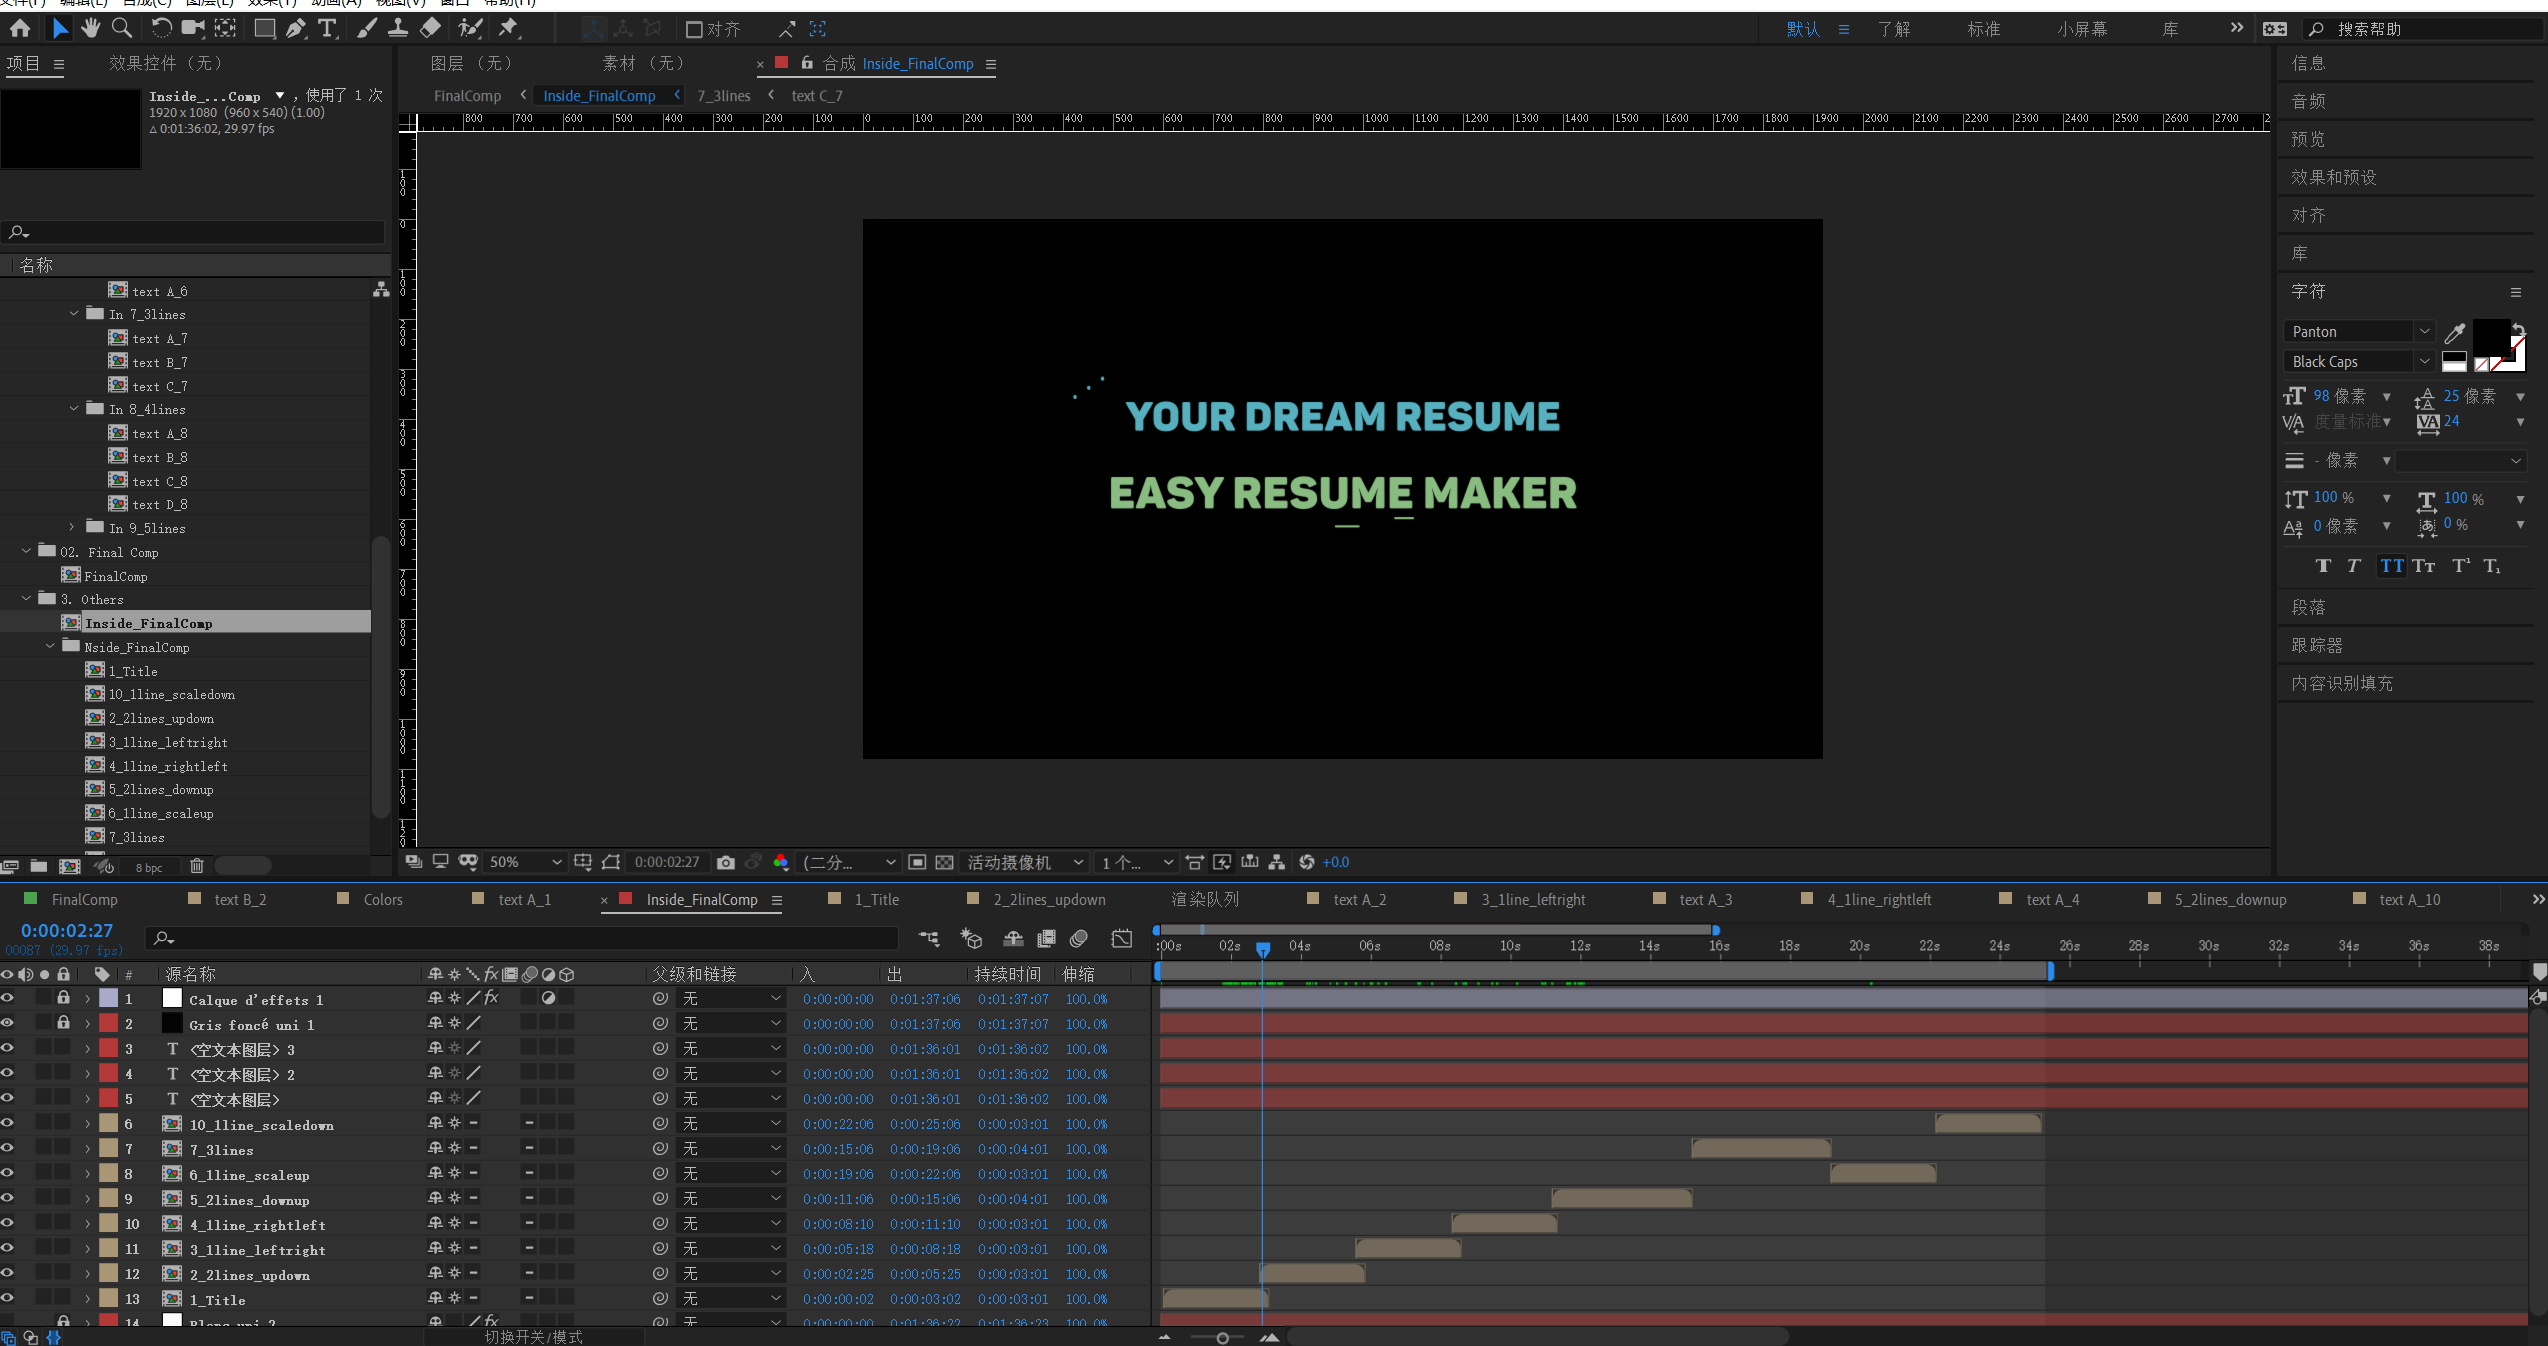
\includegraphics[scale=0.2]{figures/ae.png}
	\caption{After Effect}
	\label{fig:6}
\end{figure}
Since this lottie tool is so new, we think we have made it pretty far ahead of the curve in terms of SVG usage.

	\end{itemize}
	\subsection{Server Side}
	\subsubsection{Server}
	\subsubsection{Database}
	\subsubsection{Dynamic pages}
	
	% --------------------
	% --------------------
	\section{Working practices of the group}
	% --------------------
	We used GitHub technology for remote collaboration, with Tao Xu handling the backend technology and Yinan Yang is in charge of front-end technology. Our project address is \href{https://github.com/Nonac/webtech}{https://github.com/Nonac/webtech}.The screenshot below reflects the progress of our project.
	
	\begin{figure}[H]
		\centering
		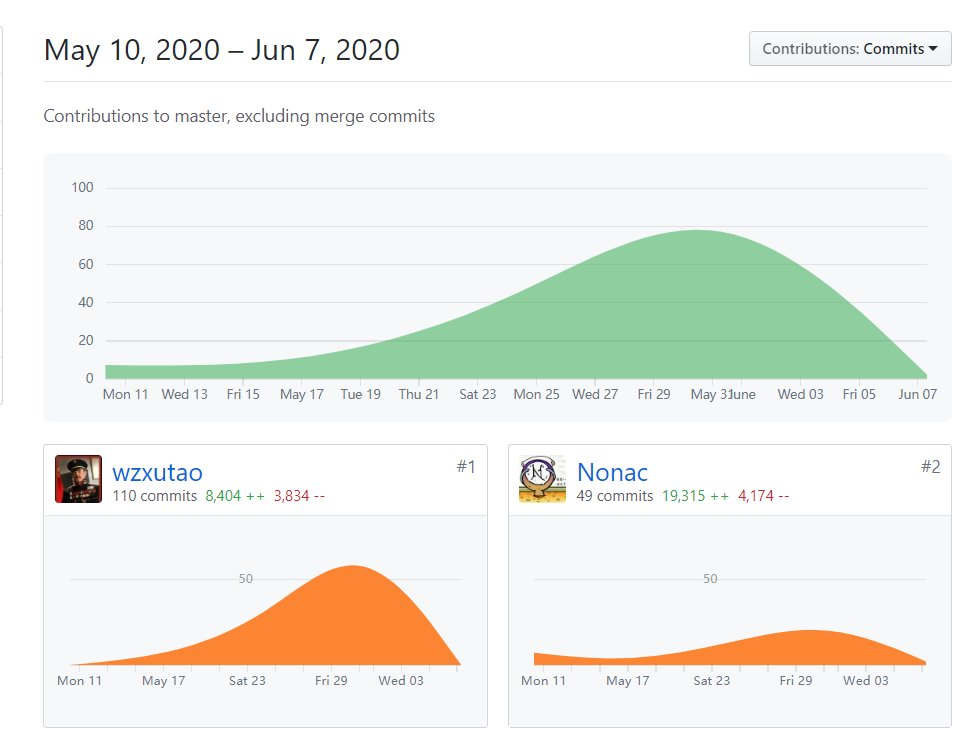
\includegraphics[scale=0.7]{figures/github.png}
		\caption{After Effect}
		\label{fig:15}
	\end{figure}
	
	% --------------------
	
\end{spacing}	
	
\end{document}